% !TeX encoding = UTF-f

%===============================================================================
% Font options are:
%   plain (default), serif (uses Palladio), sans-serif (uses Paratype Sans)
% Layout options are:
%   article (default, no chapters), book (for longer texts, offers \chapter)
% Paragraph options are:
%   noparskip (default, no spacing between paragraphs), parskip (spaced)
\documentclass[serif,article,noparskip]{agse-thesis}
\usepackage{amsmath}

% Global parameters, replace with actual values.
\newcommand{\thesisTitle}{Implementation of a Software to detect the different Retangles in Images created by Piet Mondrian}
% -> You may use \par (but not \\) to format the title. If you do so, you'll
%    need to manually set the 'pdftitle' attribute below.
\newcommand{\studentName}{Finn Pauls}
%===============================================================================

\hypersetup{pdftitle={\thesisTitle}}
\hypersetup{pdfauthor={\studentName}}

\begin{document}

\coverpage[
    student/id=4788442,
    student/mail=finn@inf.fu-berlin.de,
    thesis/type=Bachelorarbeit,            % optional, default: Bachelorarbeit
    thesis/group={Arbeitsgruppe Theoretische Informatik},
    thesis/advisor={Martin Skrodzki},           % optional
    thesis/examiner={Prof. Wolfgang Mulzer},
    thesis/examiner/2={Prof. Dr. Konrad Polthier}, % optional
    thesis/date=\today,                    % optional, default: \today
   %title/size=\LARGE,      % set this value to overwrite automatic font size
   %abstract/separate       % toggle this to move the abstract to its own page
]
{ Abstract TBD}

% !TeX encoding = UTF-8
\subsection*{Eidesstattliche Erklärung}

Ich versichere hiermit an Eides Statt, dass diese Arbeit von niemand anderem
als meiner Person verfasst worden ist. Alle verwendeten Hilfsmittel wie
Berichte, Bücher, Internetseiten oder ähnliches sind im Literaturverzeichnis
angegeben, Zitate aus fremden Arbeiten sind als solche kenntlich gemacht. Die
Arbeit wurde bisher in gleicher oder ähnlicher Form keiner anderen
Prüfungskommission vorgelegt und auch nicht veröffentlicht.\\

\thesisDate \\

\studentName


\cleardoublepage

\tableofcontents

\cleardoublepage

\mainmatter

\section{Introduction}

% Introduce general problem area?

\subsection{Piet Mondrian}

The oeuvre of Piet Mondrian (1872-1944) consists of figurative paintings as well
as abstract compositions. Up until 1910 his works only depicted naturalistic
scenes like churches, trees, windmills or landscapes. From 1911 onwards his
paintings remain representational but are increasingly painted in a more
abstract way.

Around 1914 his compositions begin to be purely abstract and in 1917 he cofounds
the artistic movement and group \textit{De Stijl} also known as
\textit{Neoplasticism}. One of the primary objectives of the group is to reform
art by "abolishing natural form" \cite{wiki:manifest} altogether.

At some point around 1920 Mondrian further restricted his compositional elements
to rectangles and straight black lines. The lines were only allowed to run
horizontally or vertically. Only primary colors (red, blue and yellow) and
non-colors (black, white and grey) were allowed to be used.

Another founding member of \textit{De Stijl}, Georges Vantongerloo, used methods
inspired from mathematics for his compositions. One example of this is his
painting "Composition Derived from the Equation y = -ax2 + bx + 18".

Mondrian on the other hand is known to only use intuition when creating his
works, moving compositional elements for weeks, seeking a balanced composition,
until he was satisfied with the result.
% Find Citation, better
% Deicher, S., (1995), Mondrian, Taschen (Koln), 1995 - Mondrian obsessed with positioning. he spends long periods of time shifting a single line back and forth within a couple of millimetres, believing that a precise positioning was essential for capturing an aesthetic order that was “free of tension”. Australian

% TODO: Avoid Symmetry

Still many people have been interested in the question if Mondrian's
non-figurative paintings utilize certain compositional rules or techniques that
the painter might have used unconsciously. One approach that only became
feasible in the 1960s is to recreate art that resembles Mondrian's composition
using computers.

\subsection{Related Works}

There have been multiple attempts at creating art that resembles Mondrian's
compositions using computers. Feijs (2004)\cite{Feijs2004} presents different
techniques for generating images resembling non-figurative Mondrian paintings
from different periods. He concludes that different kinds of algorithms for
generating images can be used to formalise the distinction between different
types of Mondrian paintings.

Skrodzki and Polthier (2018) \cite{Skrodzki2018} use computer models to generate
Mondrian-inspired three-dimensional pieces using the KdTree data structures.
They note however that while their results are similar to Mondrian paintings,
they do not always resemble Mondrian paintings since proportions are randomly
chosen and not carefully.

There have been attempts to study the organisation and proportions of the
compositional elements used by Mondrian. In 1968 Hill \cite{Hill1968} analysed
the network topology of Mondrian's paintings. One of his findings shows the
avoidance of symmetry on a structural level. He also criticised earlier work for
inaccuracy of measurement and the lack of statistics and called for a more
substantiated analysis of the paintings.

Some sources \cite{bouleau1963,bergamini1980} suggest that Mondrian used golden
rectangles in his paintings. A golden rectangle is rectangle, where the ratio
between the sides length is the golden ratio $\phi \approx 1.618$. Other authors
however \cite{Livio2002,Markowsky1992} refuse those claims, finding fault with
the lack of evidence, which consists mostly just of exemplary superimposing
golden rectangles on paintings.

Despite this disagreement there have been very little attempts on actually
evaluating this question statistically. In a poster from 2017, Tanaka and
Miyanaga \cite{Tanaka2017} examine the use of rectangle ratios, specifically the
golden and silver ratio, in 10 late Mondrian paintings. They conclude that
Mondrian actually had a preference for the silver ratio $\delta_S = \approx 2.414$ instead.

However to the authors knowledge there is no publication examining the question of
the use of certain special ratios on Mondrian's paintings with a larger data
set.

% TODO: Could also be in discussion?
% More motivational, could be easier done with our program
% http://faculty.philosophy.umd.edu/jhbrown/mondriansbalance/index.html#19
% "The lesson is that we must exploit digital technology to the full and set Mondrian's
% designs into the relevant space of possibilities if we are ever to put judgments
% of aesthetic balance on a firm footing – which at present they are clearly not."
% "Such findings also suggest that we can put the formalist sector of aesthetic
% response on a firm footing only by much more extensive and rigorous
% experimentation with transforms of existing designs"

\subsection{Scope of the Thesis}

Providing numeric data to close the lack of foundation for analysis on the
neo-plastic compositions by Mondrian is the main objective of this thesis. The
goal is to create a program that uses methods of Computer Vision to extract the
compositional elements from images of the paintings. The program is restricted
to paintings from 1920-1937 that also always use black lines to separate the
rectangles and are not drawn on a diamond canvas.

% !TeX encoding = UTF-8

\section{Fundamentals} \label{fundamentals}

In this section we will specify the different definitions used for
conceptionalizing the program (\ref{definitions}). We are also going to present
different existing methods and algorithms that were used (\ref{used}).
Lastly we are going to outline the concept for detecting the structure of rectangles
in Mondrians abstract paintings (\ref{concept}).

\subsection{Definitions} \label{definitions}

We define an Image $X$ with width $w$ and height $h$ to be the set $I$.
$$I = \{p_{xy} | x \in \{1,2, \dots w\}, y \in \{1,2, \dots h\} \}$$
A RGB Image $I$ is an Image with the following  $p_{xy}$: $$p_{xy} = (r_{xy}, g_{xy}, b_{xy}) \in \{0,1,...,255\} \times
\{0,1,...,255\} \times\{0,1,...,255\}$$ A Greyscale image is an Image with
$p_{xy} \in \{0,1, \dots 255\}$ and a Binary Image $B$ is an Image with $p_{xy} \in \{0,1\}$ where we also refer to
$0$ as \textit{black} and $1$ as \textit{white}

\subsection{Used Algorithms and Methods} \label{used}

For preprocessing the images, a combination of methods are used: \textit{Image
Morphology}, \textit{Thresholding}, \textit{Contrast Limited Adaptive Histogram
Equalization (CLAHE)} and \textit{Masks}. These algorithms are provided by the
Python distribution of the Open Source library OpenCV \cite{opencv_library}.

\subsubsection{Image Morphology}

Image Morphology is based on Mathematical Morphology from the mathematical field
of set theory. We are going to present two basic morphological operators
commonly used in image processing without going into detail of their
mathematical definition. A more formal definition and further reading can be
found in Aguardo (2012) \cite{Aguardo2012}.

Given a binary image $B$ and a smaller binary image $B_s$ called the
\textit{Structuring Element}, with a dedicated center point $c \in B_s$ we can
apply the basic operations \textit{Erosion} and \textit{Dilation}.

% Maybe add image about Erosion

The Erosion $B \ominus B_s$ is equivalent to iterating through all of the white
pixels of $B$ and only keeping them if all of the points of $B_s$ translated
by its center point $c \in B_s$ to this position are fully included in $B$.
Therefore the white areas in $B$ are reduced . \cite{Smith1997}

Similarly for the Dilation operation  $B \oplus B_s$ , the center point of the
Structuring Element is translated to every pixel $p \in B$. For each of these
pixels all the neighbouring pixels that intersect with the translated $B_s$ are
turned white. The total area of white pixels is increased. \cite{Smith1997}

Image Morphologies have multiple uses like increasing certain areas for better
recognition or separating larger shapes of an image. In our case they will be
helpful for correcting interruptions in the black lines of the image as well as
for separating black areas that are bigger than typical lines.

\subsubsection{Thresholding}

Thresholding $T(G) = \{t_{xy}\ \in {0,1} | g_{xy} \in G\}$ is a process for turning a greyscale image $G$
with pixels $g_{xy}$ into a binary image $B$ using a threshold $t \in
0,1,\dots255$. Each pixel $t_{xy}$ is assigned a black or white value given
whether it is below or above the threshold.

\begin{equation}
  t_{xy} =
  \begin{cases}
    0 & \quad  \text{if}  \quad g_{xy} \leq t\\
    1  & \quad \text{if}  \quad g_{xy} > t
  \end{cases}
\end{equation}

\subsubsection{Contrast Limited Adaptive Histogram
Equalization (CLAHE)}

A \textit{Histogram} of an image is the distribution of brightness values in an
image. \textit{Histogram equalization} is the process of adjusting the contrast
of an image using the Histogram. Global histogram equalization changes the
brightness of each pixel in the image using the overall histogram of the image.
\cite{ShapiroLindaG2001Cv}

\textit{Adaptive histogram equalization (AHE)} on the other hand only uses the
histogram of a specified area around any given pixel to adjust its brightness.
It therefore is better able to increase the local contrast.

However \textit{AHE} tends to overamplify noise in an image. Fairly uniform
regions of the same brightness have high histogram pieaks and are turned into
noisy patterns.  \textit{Contrast Limited Adaptive Histogram Equalization
(CLAHE)} limites this effect by setting a maximum value for the values of the
histogram. \cite{Pizer1987}

\subsubsection{Masks}

Masks operations are similar to elementary arithmetics. Each pixel $a_{xy}$ in
one image  $X_a$ is added, substracted, multiplied or divided with $b_{by}$ of
another image $X_b$. For example the operation $X_a + X_b$ denotes the set
$\{\mathrm{min}(255, p_{xy} + q_{xy}) | p_{xy} \in X_a, q_{xy} \in X_b\}$. For our purposes we only
use addition and substraction.

% TODO: Possibly try to use Opening operation again and explain it here

\subsection{Concept} \label{concept}

%TODO: Define mondrian paintings in our context

Our aim for the detection algorithm is to take a cropped Mondrian painting as
an input and detect all the rectangles in it as well as their colors.

The input is an RGB Image $I_1$ of a Mondrian painting. The expected output is a
list of rectangles with their position, sizes and color as they are
conceptionally seen in the painting. All rectangles combined are expected to
exactly cover the area of the input image in a way that the original could be
dissected into this set of rectangles. The thick black lines in the paintings
are seen as one-dimensional lines that are positioned in the middle of the
detected thicker lines.

The algorithm itself can be separated into two different phases: Image
preprocessing (\ref{preprocessing}) and the recognition of rectangles (\ref{rectangles}).

The goal of the first preprocessing phase is to obtain a binary image in which
black represent the lines of the painting while white represents the inner area
of the rectangles. The different steps of the preprocessing phase are visualized
in Figure \ref{fig:preprocessing}.

The second phase then takes this binary image and returns a list of found
rectangles. Additionally, for recognizing the colors of the rectangles, the
original input image is used.

\subsubsection{Image preprocessing} \label{preprocessing}

\begin{figure}
  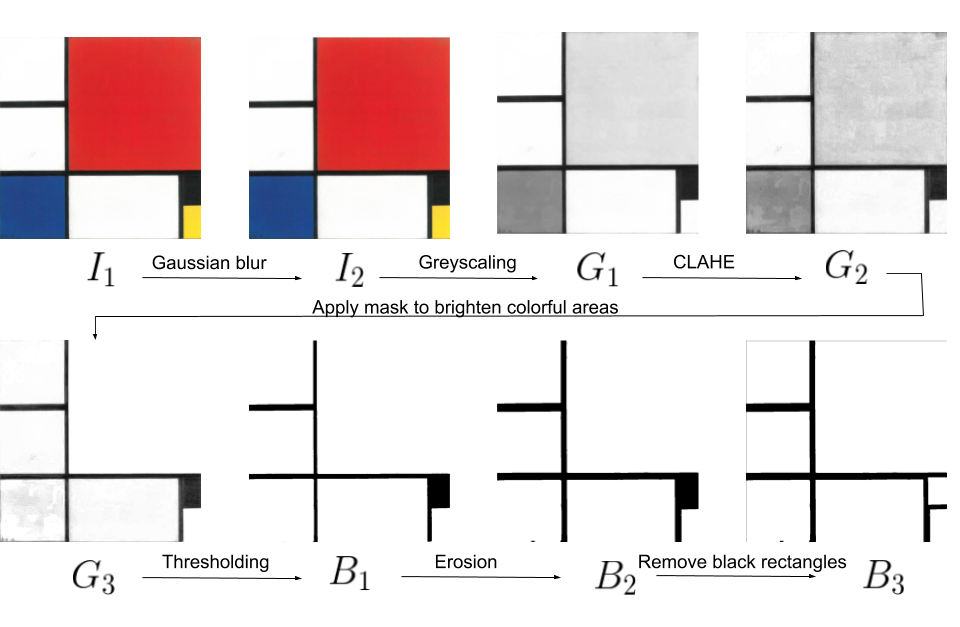
\includegraphics[width=\linewidth]{images/preprocessing_steps.png}
  \caption{Preprocessing Steps on \textit{Composition II in Red, Blue, and Yellow
  from 1929}}
  \label{fig:preprocessing}
\end{figure}

At first, a Gaussian blur is applied to the input RGB Image $I_1$ to reduce
artifacts that the input images might include, we call the result of the blur
$I_2$. These artifacts might be craquelure or fading of darker areas in the
paintings. But they might also be results of the photography and scanning the
images.

Next, the RGB input image is decomposed into a Greyscale Image $G_1$ by using
the maximum value of the RGB triplet for each pixel in $I_2$:
$$G_1 = \{p_{xy} \in \{0,\ldots,255\} \mid (r_{xy},g_{xy},b_{xy})\in I_2\text{ and }p_{xy}=\max\{r_{xy},g_{xy},b_{xy}\}\}$$.

To normalize the brightness distribution of $G_1$ and increase the contrast of
the darker regions, we now apply histogram equalization to $G_1$. For this we
use \textit{Contrast Limited Adaptive Histogram Equalization (CLAHE)}. In
contrast to non-adaptive and ordinary adaptive histogram equalization
algorithms, this prevents the overamplification of noise as reasoned above. We
call the result of the equalization $G_2$. \cite{Pizer1987}

After the normalization is applied, we further brighten colorful areas of the
image to make them stand out against the black areas of the paintings. This way,
for example, darker blue areas can be better distinguished from black areas.
Since the difference between the maximum and the minimum value of the RGB
triplet is related to the colorfulness of a pixel, we calculate this for every
pixel of the input image. The resulting Mask $G_m$ from this calculation is added to
the contrast-normalized image $G_3 = G_2 + G_m$.

Now the image $G_3$ with the elements $g_{xy}$ is converted into a binary image
using Thresholding $B_1 = T(G_2)$. The threshold value $t$ needs to be chosen
as such as its optimally separating between the darker lines an the lighter
rectangles in the image. See \ref{parameter} for how that value was determined
in praxis.

Since the thresholding step might leave some interruption in the black lines, we
reduce the white areas of the image: An Erosion $B_2 = B_1 \ominus B_e$ is
applied. In this case, the structuring element $B_e$ is a $N\times N$ binary
Image. Using the Erosion some accidental interruptions in the lines can be
restored. However choosing a Structuring Element that is too big, might
result in loss of information by filling smaller white rectangles black.
Therefore the size $N$ needs to be chosen carefully.

The resulting image $B_2$ now separates the darker parts of the image fairly
well. However, we are only interested in black lines, but Mondrian paintings
also include filled black rectangles. To remove these black rectangles, we
create a mask that applies a Dilation $B_m = B_2 \oplus B_d$ with a larger
Structuring Element $B_d$ compared with $B_e$ on the image. The size of $B_d$ is
chosen in a way that most of the lines in the paintings are removed, only
leaving inner areas of black rectangles. The resulting mask $B_m$ is then
removed from the image of the last step $B_3 = B_2 - B_m$. Hence only the
outlines of the black rectangles, as well as the black lines, remain in $B_3$.

\subsubsection{Detection and recognition of rectangles} \label{rectangles}

Since the rectangles in the painting are defined by the horizontal and
vertical lines in the image, the detection starts by finding all of those lines
in the output binary image $B_3$ from the previous phase.

% TODO: Define all the different termini (lines, etc.)

To find horizontal lines $H$, the image is scanned vertically line by line. We
iterate through the pixels of each horizontal line. Uninterrupted sequences of
black pixels are added to a list of horizontal lines. Only sequences with a
specified minimum length $\ell$ are added (See \ref{parameter} for details).
The minimum length should be slightly larger than the maximum width of the lines
in the image. Vertical lines $V$ are recognized respectively by iterating
through the lines from left to right.

% As a first step to find horizontal lines $H$, consecutive black pixels in every
% row of the image are considered a line if at least $l$ of them occur without
% interruption. The minimum length should be slightly larger than the maximum
% width of the lines in the image. The same way a set of vertical lines $V$ can be
% obtained for every column. This is the equivalent of applying a lossy run-length
% encoding once horizontally and once vertically.

However, this means that what we perceive as one horizontal line in the painting
is now recognized as multiple lines next to each other. For example, a line that
is 50 pixels wide would be recognized as 50 lines. Therefore as a next step
parallel lines close to each other are merged into a single line. As long as
parallel lines are within a certain distance $d$ from each other, they are merged
into one line. For horizontal lines, the resulting line will have the average
$y$ value of all those lines and the minimum and maximum $x$ values as starting
and end points.

From our conceptional view on Mondrian paintings, the ends of lines always touch
another line or the edge of the painting. However, the lines that we reduced now
might overlap slightly or not even connect to the next line.

Now we consider the two ends of every horizontal line $h \in H$. For each end $e =
(x_e,y_e)$ we find the closest vertical line $v \in V$ that could touch $e$ by only
translating it horizontally.

Since a rectangle is defined by the black lines in the paintings as well as the
edges of the painting, we add the lines of the edges to the $H$ and $V$ as well.

%TODO: How are they identified as top-left?

All lines should now represent the structure of the painting. What we want as
our output though is a list of rectangles. Every rectangle in the image can be
defined through a set of four different corners: top-left, top-right,
bottom-left and bottom-right. These corners are always intersections of two
lines, either crossing or touching. We determine the corners and their types by
iterating through the lines.

After this, four different corners are combined into a rectangle by finding
matching corners. This is done by iterating through the top-left corners $(x,y)$
and finding the closest top-right corner to the right $(x_r, y)$ and the
closest bottom-left corner below $(x, y_b)$. The rectangle is then defined by
the position of the top-left corner and its width and height
$(x,y,x_r-x,y_b-y)$.

For this list of rectangles, we determine the colors of the rectangles. For this
purpose, we clip the rectangle from the original image and determine the average
color or the selection. This color is then reduced to either black, white, red,
blue or yellow.

\section{Implementation} \label{implementation}

In this section, I want to present our implementation of the above-described
concept. We are going to show how the software is structured
(\ref{structure}), discuss challenges in performance (\ref{performance}) and
explain how parameters were chosen (\ref{parameter}).

The algorithm was implemented in Python 3.7 using the \textit{OpenCV} and
\textit{NumPy} libraries. OpenCV provided the different image processing methods
described in \ref{used} as well as other methods for reading, writing and
manipulating image files. NumPy, which is part of the SciPy package, is a
package for scientific numerical computing \cite{scipy}.
% Images in OpenCV are represented as three-dimensional NumPy arrays. The first
% two dimensions of this array encode the positions of pixels in the image, while
% the third dimension encodes the three color values.

\subsection{Structure} \label{structure}

The main algorithm was implemented in a function \texttt{process\_image}. This
function takes a 3-dimensional array representing the image as an input and
outputs a tuple. The first element of that tuple is the actual output, a list of
rectangles found in the image. The second element is a list of images, which
represent different steps of the algorithm and are artifacts meant for debugging
and feedback. Each rectangle in the list carries information on position, dimensions
and color.

% TODO: Is the debug stuff important? Maybe have their own section for it?

Another function called \texttt{run\_pipeline} reads a list of images from a
given input directory and feeds them into \texttt{process\_image}. Each of the
debug images given is saved to disk in an output directory. The data from the
rectangles is encoded in a \textit{JSON} file for each image. \textit{JSON} was
chosen, since it is a widespread flexible data-interchange format that is also
human-readable. An example for such a \textit{JSON} file can be seen in Figure
\ref{fig:json}.

\begin{figure}
\begin{minipage}{0.2\textwidth}
  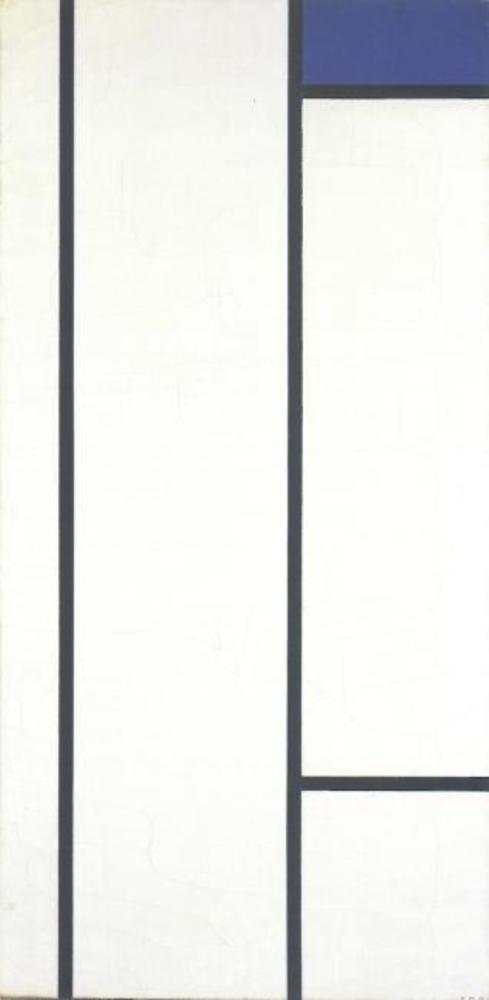
\includegraphics[width=\linewidth]{images/B244.jpg}
\end{minipage}
\begin{minipage}{0.8\textwidth}
\begin{lstlisting}
{
  "id": "B244",
  "height":1000,
  "width":489,
  "rectangles":[
    {"x":294,"y":91,"w":195,"h":691,"c":"white"},
    {"x":294,"y":782,"w":195,"h":218,"c":"white"},
    {"x":64,"y":0,"w":230,"h":1000,"c":"white"},
    {"x":294,"y":0,"w":195,"h":91,"c":"blue"},
    {"x":0,"y":0,"w":64,"h":1000,"c":"white"}
  ]
}
\end{lstlisting}
\end{minipage}
\caption{Source image and \textit{JSON} representation for \textit{Composition no. I (1934)}}
\label{fig:json}
\end{figure}


\texttt{process\_image} first calls another function \texttt{preprocessing} that
executes the steps described in \ref{preprocessing}.

Then the result of \texttt{preprocessing(image)} is used as the input for
\texttt{detect\_rectangles}. This function executes the steps described in
\ref{rectangles}. The result is a list of rectangles and their colors. As well
as images that show a visual representation of the rectangles next to the input
image. They can be used to validate the result of the algorithm.

At first \texttt{detect\_rectangles} uses \texttt{detect\_lines} to extract a
list of all vertical and horizontal pixel lines from the preprocessed image.
Then \texttt{reduce\_lines} combines parallel lines that are next to each other
into a single line. It iterates through the items in the list and looks for
neighbouring lines by iterating in another nested loop through the same list. If
a matching line is found, the line is removed from the list, so that it will not
appear in the iteration again. The loose ends of the lines are then connected by
\texttt{connect\_lines}.

As an example Listing \ref{lst:findrectangles} shows the source code of
one of the function \texttt{find\_rectangles}, which finds rectangles from a
list of top-left, bottom-left and top-right positions. The length of each of
these lists is the same and is expected to be the number of rectangles. The
program first sorts the top-right corners by their x position and the
bottom-left corners by their y position. When iterating through the top-left
corners, we know that their x position is going to be the same as the matching
bottom-left corner \texttt{bl}, but a larger y-coordinate. So we only select
these candidates from the \texttt{bottom\_left} list using an iterator
expression. Since we ordered the corners before from top to bottom, we know the
matching corner is going to be the first returned by the iterator. We therefore
only call the iterator once with \texttt{next}. The same logic is applied to
bottom-left corners. Using the coordinates of the matching top-right and
bottom-left corners, the rectangle is calculated and added to a list of
rectangles as a tuple. That list is then returned by the function.

\begin{minipage}{\linewidth}
\begin{lstlisting}[label=lst:findrectangles,caption=Function for constructing rectangles from corners]
def find_rectangles(top_left, bottom_left, top_right):
    top_right.sort(key=lambda pos: pos[0])
    bottom_left.sort(key=lambda pos: pos[1])
    rectangles = []
    for x,y in top_left:
        x2,_ = next(tr for tr in top_right if tr[1] == y and tr[0] > x)
        _,y2 = next(bl for bl in bottom_left if bl[0] == x and bl[1] > y)
        w = x2 - x
        h = y2 - y
        rectangles.append((x,y,w,h))
    return rectangles
\end{lstlisting}
\end{minipage}

\subsection{Iterative approach}

The different processing steps of the algorithm are visualized by providing
multiple output images for each input image. These images allow an inspection
of the different intermediary results created in the process.

Thes images were used to identify problems that might occur during the detection
and could then be used as a basis for the adjustment of the parameters (see
\ref{parameter}).

This visual feedback also provided insights into problems of the algorithm like
small bugs or conceptional problems. For example the preprocessing step to
increase the brightness of areas that are more colorful was introduced because
there were issues of discriminating darker blue areas from black ones. This way
the development of the algorithm could follow an iterative approach.

\subsection{Performance} \label{performance}

The performance of the algorithm was measured by timing the duration for each
image. The first implementation of the algorithm took about 1100 milliseconds per
iteration. By running timings on different parts of the processing, the
\texttt{detect\_lines} function was discovered as a bottleneck. It was
accountable for about 93 percent of the processing time.

This was the only place in the program were we iterated through all of the pixels
in the image using Python. All other operations were done using OpenCV or NumPy.
They also iterate through all of the pixels but using optimized C code.

To reduce the time of this step we decided to reimplement this function in a
compiled, more low-level language. We chose to use Rust using the \textit{rust-cpython}
library for bindings. Using the same algorithm implemented in Rust, the time of
this step was reduced from about 1020 to 40 milliseconds. The runtime of the
program could be reduced by a factor of 13.

This time could have been be further reduced by running multiple parallel
iterations over the different rows or colums. However for our purpose the
achieved time was sufficient.


\subsection{Parameter Selection} \label{parameter}

By running the program on the images and looking at the debugging output images
for the different steps, the reasonable values for the parameters of the program
can be determined.

By running the program and looking at the results of the Thresholding for each
image, comparing it to the input image, the threshold value $t = 110$ was
determined to give reasonable results.

To better fine-tune the parameters, we selected a subset of input images and
always manually changed these parameters until the result was correct. The
resulting \textit{JSON} files with the correct results were moved to another
directory \textit{detected}. Then a step was added to the program that would
always compare the computed result with the data in that directory if available.
When the result differed, it would print out a warning.

Using this output the minimum length $\ell$, the maximum width $d$ and the size of
the erosion kernel $N$ were changed to maximize the number of recognized images
from that set. The resulting parameters were $l = 60$, $d = 70$ and $N =11$.

\subsubsection{Evaluation of Tools}

Reflecting about the used tools, I would definitely choose OpenCV again. It
supports a variety of established computer vision algorithms, is well documented
and has a variety of learning resources. Since OpenCV primarily supports C++ and
Python interfaces, the programming language choice was one of these options.
While using the compiled language C++ could have increased performance over the
interpreted Python, it would also have decreased productivity.
Python's readibility and user-friendly data-structures made it a good choise for
an iterative development.

% !TeX encoding = UTF-8
\section{Results} \label{results}

 The image selection was restricted to paintings 1920-1937. There are 178 works
 listed in the \textit{Catalogue Raisonn{\'e}} \cite{joosten1998} for that time
 period. 28 of those were sketches, unfinished work or not a painting. Of the
 remaining 12 were drawn on a diamond-shaped canvas and for 20 paintings was
 either no or only a greyscale image available. The remaining 178 images were
 scanned and subsequently cropped so that only the painting and no frame was
 visible.  The images were scaled so that the longer side would be 1000
 pixels. The images were then processed by the detection program and subsequently
 checked for accuracy by comparing the result with the original. The resulting
 dataset consists of 1316 rectangles and their respective size, colors, and
 paintings.

Some explorative analysis about the use of color (\ref{color}) and ratios
(\ref{ratios}) was performed.

\subsection{Colors} \label{color}

On average Mondrian paintings consist of 79.7\%  and non-colors (black, white)
20.3\% colors (red, blue, yellow) ($\sigma = 17.0\%$), see Figure
\ref{fig:colors-noncolors}. The median percentage of each color appears to be
rather similar, the distribution of red however is more widespread as you can
see in Figure \ref{fig:colors-rby}.

\begin{figure}
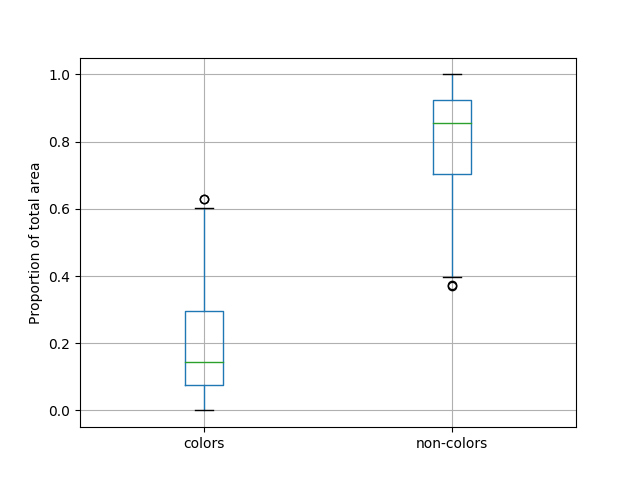
\includegraphics[width=\linewidth]{images/colors-non-colors.png}
\caption{Evident preference of non-colors in the paintings}
\label{fig:colors-noncolors}
\end{figure}

\begin{figure} 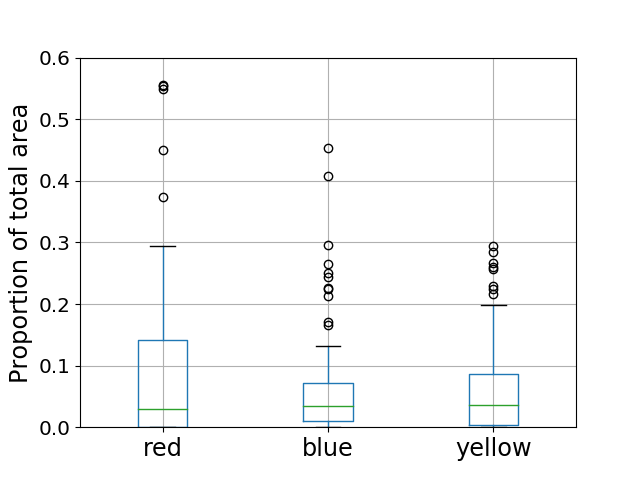
\includegraphics[width=\linewidth]{images/colors-rby.png}
\caption{Median proportion of the colors are very similar, red however has a
more wide distribution} \label{fig:colors-rby} \end{figure}

To see if different colors of rectangles have overall preferred positions in the
compositions, we assembled a dataset of all rectangles and their respective
positions, width and colors. We calculated the centers of all of these
rectangles and plotted them by color. We also visualized the estimated
probability density function of the positions using Kernel density estimation
with an Gaussian kernel selected by Scott's method \cite{Terrell1992}. The
result is given in Figure \ref{fig:kde}. The first thing you notice is that the
color red appears to have a substantial bias to the top-left corner. Similarly
blue has a slighter bias to the bottom-right corner.

\begin{figure}
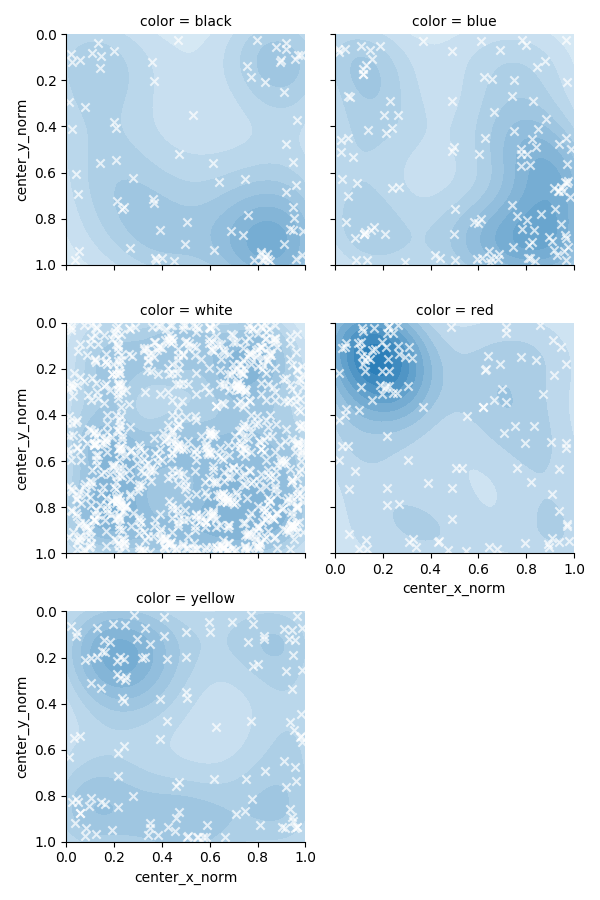
\includegraphics[width=\linewidth]{images/kernel-densities.png}
\caption{Scatter plots and KDE for each color}
\label{fig:kde}
\end{figure}

\subsection{Ratios} \label{ratios}

For all rectangles we calculated the aspect ratio of the longer to the shorter
side. Figure \ref{fig:aspect-rects} shows the estimated probability density of
the ratios and Figure \ref{fig:longer-x-shorter} shows all rectangles plotted by
their sides as well as lines for certain proposed ratios. The data does not show
peaks for the golden or silver ratio. This supports the rejection by Livio
(2002) \cite{Livio2002} and Markowsky (1992) \cite{Markowsky1992} of the golden
rectangle claim by Bouleau (1963) \cite{bouleau1963} and Bergamini (1980)
\cite{bergamini1980}.

\begin{figure}
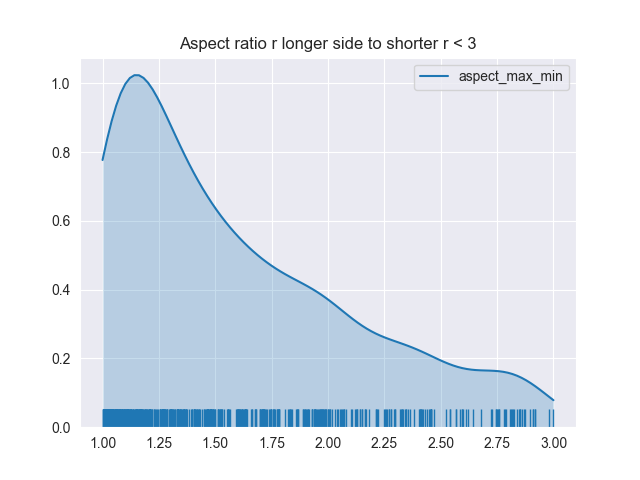
\includegraphics[width=\linewidth]{images/aspect-max-min-rects.png}
\caption{Rectangles ratio KDE}
\label{fig:aspect-rects}
\end{figure}

\begin{figure}
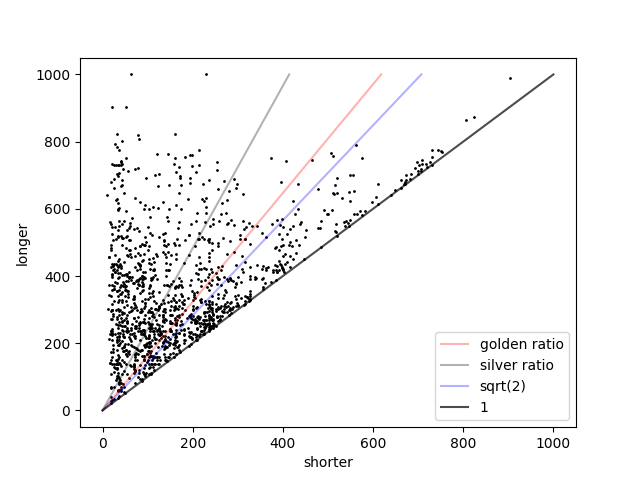
\includegraphics[width=\linewidth]{images/longer-x-shorter.png}
\caption{Rectangles longer side to shorter side}
\label{fig:longer-x-shorter}
\end{figure}


% TODO: Number of rectangles over time?
% TODO: How many paintings use all colors? How many with only one?

% !TeX encoding = UTF-8
\section{Discussion} \label{conclusion}

The developed program is able to detect rectangles in a class of abstract
Mondrian paintings. Human control and intervention are still necessary to make
sure the result is correct. By adjusting the input parameter or in some cases
manually editing the input images, all images were detected successfully. From
the dataset of all chosen images 76\% of the images could be detected without
manual intervention.

A first look at the resulting data showed some interesting finding that deserves
further investigation. The dataset that we obtained from the images will be made
freely available for other applications, from statistical analysis to machine
learning.

The data does not suggest a preferred use of the golden or silver ratio in
rectangles. There only seems to be a general tendency towards squares.
Justifying continued research into this direction should depend on findings in
the psychology of aesthetics. So far the studies about the visually pleasing
nature of golden rectangles appear to contradict each other. Perceptional
studies about the silver ratios are missing entirely. However, research in  ratios
of other components, like the positioning of lines or the size of rectangles to
each other might lead to interesting results.

In "Art and Visual Perception" Rudolf Arnheim \cite{Arnheim1965} notes that "an
object in the upper part of the composition is heavier than none in the lower;
and location at the right side makes more weight than location on the left."
Winner (1987) \cite{Winner1987} psychologically tested these principles by
showing abstract images and their horizontally or vertically flipped
counterparts. Their findings support the up-down-principles, but not the
left-right-principle.

Arnheim also notes that the color red is heavier than the color blue. A study
from \cite{Locher2005} found some support for this claim when showing
design-trained participants modified Mondrian paintings were some colors were
swopped.

It would be interesting to explore if the found preference by Mondrian to use
red in the top-left corner could be explained by a combination of these proposed
principles of balance or whether it is merely coincidental or habitual.


% Do digital idealized representation of Mondrian paintings are comparable
% to the actual paintings in terms of certain factors like perceptional balance

% TODO: Big is heavier than small (i think)

% More generally: More paintings by Mondrian, other artists of De Stijl and
% artists in general

% Color distribution numbers close to Pareto's Principle. Maybe 80% of the
% effect of the painting stem from the 20% of the colors. Psychological research?
% eye-tracking studies

\bibliography{bibliography}

% \appendix
% % !TeX encoding = UTF-8
\section{Anhang}

Quellcode der \LaTeX-Klasse \texttt{agse-thesis}:\footnote{Es ist nicht üblich,
den gesamten produzierten Quellcode bei einer Abschlussarbeit in Textform
abzugeben.}

\lstinputlisting[
    language={[LaTeX]Tex},
    morekeywords={ProvidesClass, DeclareOption, PassOptionsToClass,
        ProcessOptions, CurrentOption, LoadClass, RequirePackage, ifthenelse,
        ifcsdef, equal, definecolor, lstset, pgfkeys},
    basicstyle=\footnotesize\ttfamily,
    numbers=left,
    numberstyle=\footnotesize\ttfamily,
    stepnumber=5,
    inputencoding=utf8,
    extendedchars=true,
   literate={ä}{{\"a}}1 {ü}{{\"u}}1,
]{agse-thesis.cls}


\end{document}
